\documentclass{article}
\usepackage[utf8]{inputenc}
\usepackage[dvipdfmx]{hyperref}
\usepackage{fancyhdr}
\usepackage{caption, floatrow}

\usepackage[dvipdfmx]{graphicx}

\usepackage{mathtools}
\renewcommand{\theequation}{eq. \arabic{equation}}


\usepackage[
  style=numeric,
  citestyle=numeric,
  url=true,
  doi=false,
  isbn=false
  ]{biblatex}
\addbibresource{main.bib}


\DeclareNewFloatType{graph}{placement=H, name=Graph}
\floatsetup[graph]{capposition=bottom}


% contents below
% ------------------------------------------------------------------------------

\pagestyle{fancy}
\fancyhf{}
\rhead{Rikuo Hasegawa}
\chead{UPCSE PHYSICS Short Lab Report}
\lhead{\today}
\rfoot{p. \thepage}

\title{Newton's Rings}
\author{ Rikuo Hasegawa
  \\ Tutorial Group: C
  \\ Lab Group: C2 }

\begin{document}

\maketitle
\thispagestyle{fancy}
\vspace*{\fill}
\parbox{\linewidth}{\centering%
Date of Experiment: March 13th, 2019
}
\newpage


\section{Introduction}
\paragraph{}
The goal of this experiment was to observe the diameter of rings in Newton's Rings in order to calculate and measure the radius of curvature of a glass lens, as well as to measure the index of refraction of water.

\section{Theory}
\paragraph{}
When light hits a half-concave, half-flat lens from above, when the concave side of the lens is facing downwards on a reflective surface, we observe circular interference patterns called Newton's Rings. This is caused by a light source being partially reflected and partially refracted at the lens' surface.

The path difference is given by \eqref{eq:path_diff}

\begin{equation}\label{eq:path_diff}
  L = 2nt_m
\end{equation}

where $n$ is the index of refraction of the material in the gap between the lens and reflective surface and $t_m$ is the length of the gap between the lens and surface.

Dark circles will appear in places where the length of the gap $t_m$ are equal, so we observe circular rings.

Let $R$ be the radius of curvature of the concave lens, we can find that the diameter $d$ of the $m$th ring from the center has the relation shown in \eqref{eq:final}.

\begin{equation}\label{eq:final}
  d_{m}^{2} = (\frac{4R\lambda}{n})m
\end{equation}

Where $\lambda$ is the wavelength of the light source and $n$ is the same index of refraction from \eqref{eq:path_diff}.

In this experiment, we directly observe $d_m$ and look to measure the radius of curvature $R$ and refractive index $n$ for water.

\section{Experimental Equipment and Method}
\subsection{Apparatus}
\paragraph{}
The apparatus is shown in Figure \ref{fig:apparatus}.

\begin{figure}[h]
  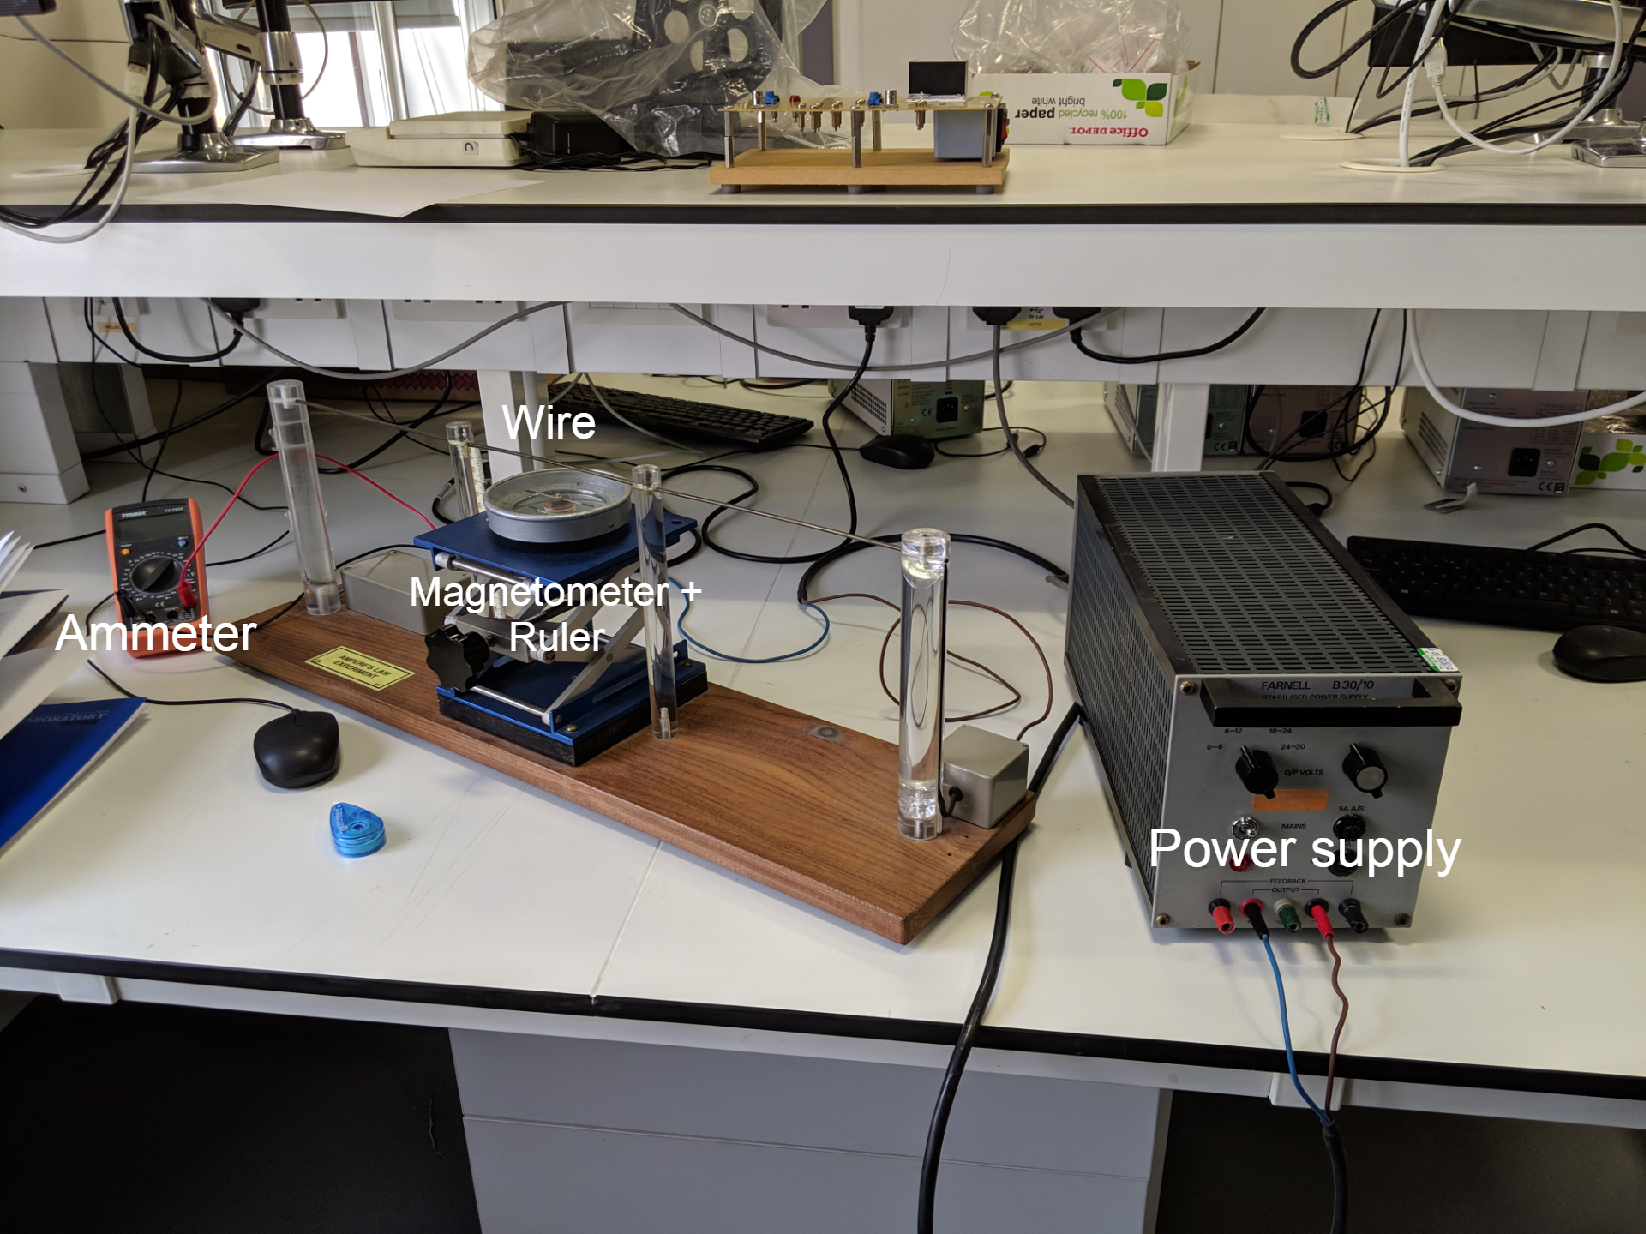
\includegraphics{./img/apparatus.pdf}
  \label{fig:apparatus}
\end{figure}

The vernier scale for the microscope which we used to measure the diameters have an accuracy of $\pm 0.005 [mm]$.

We also use a drop of water to put between the surface and lens.
Our source of monochromatic light is a sodium lamp with wavelength $\lambda$ of 589.3 [nm] \autocite{UPCSE2018}.

\subsection{Protocol}
\paragraph{}

The experiment protocol is described below:
\begin{itemize}
  \item Set the glass plate and lens as shown in Figure \ref{fig:apparatus}.
  \item Turn on the sodium lamp and locate the center of the Newton's Rings
  \item Using the vernier scale measure the radius to the left of the center for 20 rings, and repeat for the right side as well.
  \item Add some water between the lens and surface, repeat the previous step for 10 radii.
\end{itemize}

\section{Results}
\paragraph{}
Our results are summarized in Table \ref{tb:data}

\begin{table}
    \includegraphics{./img/TABLE.pdf}
  \caption{Data for diameters squared}
  \label{}
\end{table}

We plotted these values to find the gradient of the line, which should be $\frac{4R\lambda}{n}$ according to \eqref{eq:final}.

\begin{figure}
  \includegraphics{./img/grap.pdf}
  \caption{Diameter squared for water in $t_m$}
  \label{fig:water}
\end{figure}

\begin{figure}
  \includegraphics{./img/graph.pdf}
  \caption{Diameter squared for air in $t_m$}
  \label{fig:water}
\end{figure}

From this we calculated the following values for $R$:

$$
 R_{\text{air}} = 4.88 \pm 0.01 \times 10^{-1} [m]
$$
and
$$
 R_{\text{water}} = 4.85 \pm 0.14 \times 10^{-1} [m]
$$
We also calculate $n$ to be:
$$
 n = 1.34
$$

\section{Uncertainty Analysis}
\paragraph{}
Using the data analysis package for microsoft excel, we find the relative uncertainty for our measurements of $d^2$ for water to be $0.03$, and for air to be $0.01$. Comparing to the known value for the refractive index of water, $1.33$ \autocite{mohr_2016}, we find our measured refractive index to be fairly close.

\section{Discussion and Conclusion}
\paragraph{}
We find that our experiment was successful in finding the values we wished to measure with a surprising amount of accuracy.

Unfortunately, we were time constrained due to equipment troubles in the beginning followed by an interruption which consumed a significant portion of the lab time and our analysis was shallow.


\printbibliography
\end{document}
